% This is "sig-alternate.tex" V2.1 April 2013
% This file should be compiled with V2.8 of "sig-alternate.cls" May 2012
%
% This example file demonstrates the use of the 'sig-alternate.cls'
% V2.8 LaTeX2e document class file. It is for those submitting
% articles to ACM Conference Proceedings WHO DO NOT WISH TO
% STRICTLY ADHERE TO THE SIGS (PUBS-BOARD-ENDORSED) STYLE.
% The 'sig-alternate.cls' file will produce a similar-looking,
% albeit, 'tighter' paper resulting in, invariably, fewer pages.
%
% ----------------------------------------------------------------------------------------------------------------
% This .tex file (and associated .cls V2.8) produces:
%       1) The Permission Statement
%       2) The Conference (location) Info information
%       3) The Copyright Line with ACM data
%       4) NO page numbers
%
% as against the acm_proc_article-sp.cls file which
% DOES NOT produce 1) thru' 3) above.
%
% Using 'sig-alternate.cls' you have control, however, from within
% the source .tex file, over both the CopyrightYear
% (defaulted to 200X) and the ACM Copyright Data
% (defaulted to X-XXXXX-XX-X/XX/XX).
% e.g.
% \CopyrightYear{2007} will cause 2007 to appear in the copyright line.
% \crdata{0-12345-67-8/90/12} will cause 0-12345-67-8/90/12 to appear in the copyright line.
%
% ---------------------------------------------------------------------------------------------------------------
% This .tex source is an example which *does* use
% the .bib file (from which the .bbl file % is produced).
% REMEMBER HOWEVER: After having produced the .bbl file,
% and prior to final submission, you *NEED* to 'insert'
% your .bbl file into your source .tex file so as to provide
% ONE 'self-contained' source file.
%
% ================= IF YOU HAVE QUESTIONS =======================
% Questions regarding the SIGS styles, SIGS policies and
% procedures, Conferences etc. should be sent to
% Adrienne Griscti (griscti@acm.org)
%
% Technical questions _only_ to
% Gerald Murray (murray@hq.acm.org)
% ===============================================================
%
% For tracking purposes - this is V2.0 - May 2012

\documentclass{sig-alternate}

\setlength{\paperheight}{11in}
\setlength{\paperwidth}{8.5in}
\usepackage[
  pass,% keep layout unchanged
  % showframe,% show the layout
]{geometry}
\usepackage{pgfplots}


\begin{document}

% Copyright
\setcopyright{waclicense}


%% DOI
%\doi{10.475/123_4}
%
%% ISBN
%\isbn{123-4567-24-567/08/06}
%
%%Conference
\conferenceinfo{Web Audio Conference WAC-2021,}{July 5--7, 2021, Barcelona, Spain.}
\CopyrightYear{2021} % Allows default copyright year (20XX) to be over-ridden - IF NEED BE.
%\crdata{0-12345-67-8/90/01}  % Allows default copyright data (0-89791-88-6/97/05) to be over-ridden - IF NEED BE.
% --- End of Author Metadata ---

\title{Functional Reactive Programming and the Web Audio API}
%\subtitle{[Extended Abstract]
%\titlenote{A full version of this paper is available as
%\textit{Author's Guide to Preparing ACM SIG Proceedings Using
%\LaTeX$2_\epsilon$\ and BibTeX} at
%\texttt{www.acm.org/eaddress.htm}}}
%
% You need the command \numberofauthors to handle the 'placement
% and alignment' of the authors beneath the title.
%
% For aesthetic reasons, we recommend 'three authors at a time'
% i.e. three 'name/affiliation blocks' be placed beneath the title.
%
% NOTE: You are NOT restricted in how many 'rows' of
% "name/affiliations" may appear. We just ask that you restrict
% the number of 'columns' to three.
%
% Because of the available 'opening page real-estate'
% we ask you to refrain from putting more than six authors
% (two rows with three columns) beneath the article title.
% More than six makes the first-page appear very cluttered indeed.
%
% Use the \alignauthor commands to handle the names
% and affiliations for an 'aesthetic maximum' of six authors.
% Add names, affiliations, addresses for
% the seventh etc. author(s) as the argument for the
% \additionalauthors command.
% These 'additional authors' will be output/set for you
% without further effort on your part as the last section in
% the body of your article BEFORE References or any Appendices.

\numberofauthors{1} %  in this sample file, there are a *total*
% of EIGHT authors. SIX appear on the 'first-page' (for formatting
% reasons) and the remaining two appear in the \additionalauthors section.
%
\author{
  % You can go ahead and credit any number of authors here,
  % e.g. one 'row of three' or two rows (consisting of one row of three
  % and a second row of one, two or three).
  %
  % The command \alignauthor (no curly braces needed) should
  % precede each author name, affiliation/snail-mail address and
  % e-mail address. Additionally, tag each line of
  % affiliation/address with \affaddr, and tag the
  % e-mail address with \email.
  %
  % 1st. author
  \alignauthor
  \name{Mike Solomon}
  \affaddr{klank.dev}
  \email{mike@meeshkan.com}
  \date{21 December 2020}
}
% Just remember to make sure that the TOTAL number of authors
% is the number that will appear on the first page PLUS the
% number that will appear in the \additionalauthors section.

\maketitle
\begin{sloppypar}
  \begin{abstract}
    Functional Reactive Programming (FRP) is a way to model discrete and continuous signals using \texttt{events}, which carry information corresponding to a precise moment in time, and \texttt{behaviors}, which represent time-varying values. This paper shows how the behavior pattern can be used to build sample-accurate interactive audio that blends the WebAudio API with other browser-based APIs, such as mouse events and MIDI events.  It will start by presenting a brief history of FRP as well as definitions of polymorphic behavior and event types.  It will then discuss the principal challenges of applying the behavior pattern to WebAudio, including named audio units, front-loaded evaluation, and scheduling precise temporal events using different clocks.
  \end{abstract}


  %
  % The code below should be generated by the tool at
  % http://dl.acm.org/ccs.cfm
  % Please copy and paste the code instead of the example below.
  %
  %\begin{CCSXML}
  %<ccs2012>
  %<concept>
  %<concept_id>10010520.10010553.10010562</concept_id>
  %<concept_desc>Computer systems organization~Embedded systems</concept_desc>
  %<concept_significance>500</concept_significance>
  %</concept>
  %<concept>
  %<concept_id>10010520.10010575.10010755</concept_id>
  %<concept_desc>Computer systems organization~Redundancy</concept_desc>
  %<concept_significance>300</concept_significance>
  %</concept>
  %<concept>
  %<concept_id>10010520.10010553.10010554</concept_id>
  %<concept_desc>Computer systems organization~Robotics</concept_desc>
  %<concept_significance>100</concept_significance>
  %</concept>
  %<concept>
  %<concept_id>10003033.10003083.10003095</concept_id>
  %<concept_desc>Networks~Network reliability</concept_desc>
  %<concept_significance>100</concept_significance>
  %</concept>
  %</ccs2012>
  %\end{CCSXML}
  %
  %\ccsdesc[500]{Computer systems organization~Embedded systems}
  %\ccsdesc[300]{Computer systems organization~Redundancy}
  %\ccsdesc{Computer systems organization~Robotics}
  %\ccsdesc[100]{Networks~Network reliability}
  %
  %
  %%
  %% End generated code
  %%
  %
  %%
  %%  Use this command to print the description
  %%
  %\printccsdesc
  %
  %% We no longer use \terms command
  %%\terms{Theory}
  %
  %\keywords{ACM proceedings, \LaTeX, text tagging}

  \section{Introduction}
  Functional Reactive Programming (FRP) was first introduced as Functional Reactive Animation\cite{elliott1997functional} (Fran) as a way to model animate physical phenomena using Hugs, a now-defunct variant of Haskell.  Since then, a number of Haskell libraries, such as \textit{reactive-banana} and \textit{Elerea}, have provided robust implementations of FRP that are used in a number of time-based domains, including animation, user interface implementation, and signal processing.  Newer libraries such as \textit{Yampa} implement a point-free approach using the \textit{arrow} pattern, which provides a group of combinators that create a monadic context around values so that time is ``carried'' through a computation.  \textit{Yampa} has seen considerable traction in the audio community, including actings as the basis for a modular synthesizer.\cite{giorgidze2008switched}  As the need emerged to mix more heterogeneous signals and to use programming languages with varying degrees of functional expressivity, multi-language projects such as ReactiveX emerged that used the combinator-based approach over a pub-sub model via observables (emitters) and subscribers.\cite{maglie2016reactivex} Some projects, like Elm, make FRP primitives first-class citizens\cite{czaplicki2013asynchronous}.


  This paper will explore how FRP can be used to pilot the WebAudio API. It will use PureScript, a web-friendly dialect of Haskell, and a set of FRP libraries with syntax close to the original \textit{Fran} implementation.  It will start by presenting the two basic FRP types --- \texttt{Event} and
  \texttt{Behavior} --- and will the show how these can be translated into calls to the WebAudio API.

  The \texttt{Event} type is parameterized over a single type variable \texttt{a} that represents the type of an event, ie \texttt{MouseClick} or \texttt{KeyboardPress}.  The signature for an event is as follows:

  \begin{verbatim}
newtype Event a =
  Event ((a -> Effect Unit) -> Effect (Effect Unit))
       \end{verbatim}

  Here, the \texttt{Event} constructor takes a single argument: a function that accepts a callback and returns an unsubscribe effect. The callback of form \verb=(a -> Effect Unit)= accepts the \textit{event} with type \texttt{a} and performs any arbitrary side effect in the \texttt{Effect} monad.  This callback is called with the event payload, such as a key value or mouse coordinates.  The return value of \texttt{Effect (Effect Unit)} is an unsubscribe effect.  The double-effect acts as a closure so that the unsubscribe operation is not performed immediately but rather is passed to the consumer to be called at a later time, ie in the following manner:

  \begin{verbatim}
main :: Effect Unit
myEvent = do
  -- unsub is now Effect Unit after being called
  -- as part of the `bind` operation
  unsub <- makeEvent
  -- do some things, then return unsub
  -- which is Effect Unit - the type of `main`
  -- in PureScript and Haskell (although it is
  -- called IO in Haskell)
  unsub 
\end{verbatim}

  When the unsubscribe effect is called, the callback no longer receives events emitted by a source.

  With \texttt{Event}, there is no notion of time.  \texttt{Behavior}, on the other hand, introduces a notion of \textit{sampling} an arbitrary value \texttt{b} based on a known entity \texttt{a}. While behaviors can be parameterized for any event type, it is customary to use the event definition above.
  \begin{verbatim}
newtype ABehavior event a =
  ABehavior (forall b. event (a -> b) -> event b)

type Behavior a = ABehavior Event a
       \end{verbatim}

  For a behavior to work, it must always contain a value of type \texttt{a} that can be used in a sampling function that produces a value of \textit{any} type. For example, one common behavior is the current time, with a signature \verb=currentTime :: Behavior Number=. The current time can then be composed in an applicative fashion with other elements of a computation.  All the consumer of \verb=currentTime= knows is that it will used to construct a larger behavior that will act as an input to a rendering engine. The consumer has no idea what the type of this engine will be.  In the example below, it is used to produce a new \verb=Behavior= ten seconds in the future that can be further processed downstream or rendered by an engine.
  \begin{verbatim}
tenSecondsIntoTheFuture :: Behavior Number
tenSecondsIntoTheFuture =
  (_ + 10.0) <$> currentTime
       \end{verbatim}

  One way to think of behaviors is polymorphic procrastination.  Because consumers of behaviors do not know how they will be rendered, they must allow for the rendering to be polymorphic. This is achieved using rank-two polymorphism, or existential qualification, to assert with the type system that a \texttt{b} exists such that for all \texttt{a}, \verb=event (a -> b) -> event b=.  This delays the resolution of the polymorphic type until the end of the computation, ie the rendering phase.  The result is that behaviors can represent heterogeneous types through a computation and only specialized at the end - a feature of type-based existential qualification most commonly used in heterogeneous lists.\cite{kiselyov2004strongly} In our case, behaviors will represent time, mouse clicks, MIDI events, and a host of other input items that are blended together using the \texttt{Behavior} applicative functor.

  \section{Audio graphs as behaviors}

  Using the above definitions of the \texttt{Event} and \texttt{Behavior} types, we can construct a basic outline of an audio graph. The basic setup contains three steps:

  \begin{itemize}
    \item Subscribe to an event loop that is scheduled using the browser's \texttt{setTimeout}.
    \item In the subscription, sample the audio-graph behavior based on an arbitrary event.
    \item Use the resulting audio graph to drive the Web Audio API.
  \end{itemize}

  In pseudo-code, let's see how a behavior would look that incorporates information of if the mouse is clicked or not.  We'll use a \texttt{clicked} behavior.

  \begin{verbatim}
import FRP.Mouse(clicked, mouse getMouse)

audioGraph :: Mouse -> Behavior AudioUnit
audioGraph mouse = f <$> clicked mouse
  where
  f b = sinOsc (if b then 440.0 else 220.0)

main = do
  mouse <- getMouse
  unsub <- subscribe
    (interval 40) -- every 40 ms
    (const $ do
      event <- create -- make an arbitrary event
      audioNow <- sample_ (audioGraph mouse) event
      sendToWebAudio audioNow
    )
       \end{verbatim}

  The power of the behavior abstraction is that it enforces a clear separation between the push/pull mechanism (\verb=main=) and the building of the audio graph (\verb=audioGraph=).  This allows us to use a declarative style in the audio graph via \verb=clicked mouse= without worrying about the temporality and implementation of mouse event listeners.

  In the example above, there is some information that is propagated via behaviors (ie is the mouse \texttt{clicked}) whereas other information that is the result of an effectful computation (ie get the mouse via \texttt{getMouse}). This distinction is somewhat arbitrary: we could also write a mouse "behavior" that gets the mouse at any given time, and we could run an effectful \texttt{isClicked} computation whose result we pass to the audio graph instead of using a behavior.  In this way, FRP is a leaky abstraction.  Temporal events that are somehow ``distant'' from the calling code, like a mouse click, are often represented as behaviors because it allows for a succinct, declarative API like the one above. On the other hand, one-time events like \texttt{getMouse} as well as temporal phenomena that are tightly coupled with the calling code (like the current time of the audio clock of the context to which the calling code is associated) are often passed directly to a function.

  \section{Audio Behaviors in Examples}

  The following section contains three representative scenario of how temporal information can be used to construct audio graphs via FRP: approximate functions of time, precise functions of time, and integration over time.

  \subsection{Approximate functions of time}

  Approximate functions of time use quantized time at a given control rate. For example, on klank.dev, the default control rate is 50Hz. For many functions, such as gradual changes of amplitude and frequency, sampling at regular intervals produces the desired sonic effect.

  As an example, consider the following audio behavior\footnote{\url{https://klank.dev/?k&url=https://klank-share.s3.eu-west-1.amazonaws.com/K16086575564388849.purs&klank=https://klank-share.s3.amazonaws.com/klank16086575602675017.js}}:

  \begin{verbatim}
scene :: Number -> Behavior (AudioUnit D1)
scene time =
  pure
  ( speaker
         ((gain' (0.1 + (-0.1) * cos (0.5 * rad))
           (sinOsc $ 440.0 + 6.0 * (sin (0.1 * rad))))
         :| (gain' (0.1 + (-0.1) * cos (0.47 * rad))
           (sinOsc $ 330.0 + 4.0 * (sin (0.2 * rad))))
         : Nil
         )
  )
  where
  rad = pi * time
       \end{verbatim}

  All of the control rate variables, meaning everything dependent on time, is changing at a rate of 50 Hz, which means that the minima and maxima of the sine and cosine waves are truncated by a crude linear approximation.  That said, the control rate is sufficiently granular to produce the sound of gradually undulating waves without any perceptible artifacts.
  \begin{figure}[h]
    \caption{Discretized sine wave at the \texttt{purescript-audio-behaviors} control rate.}
    \centering
    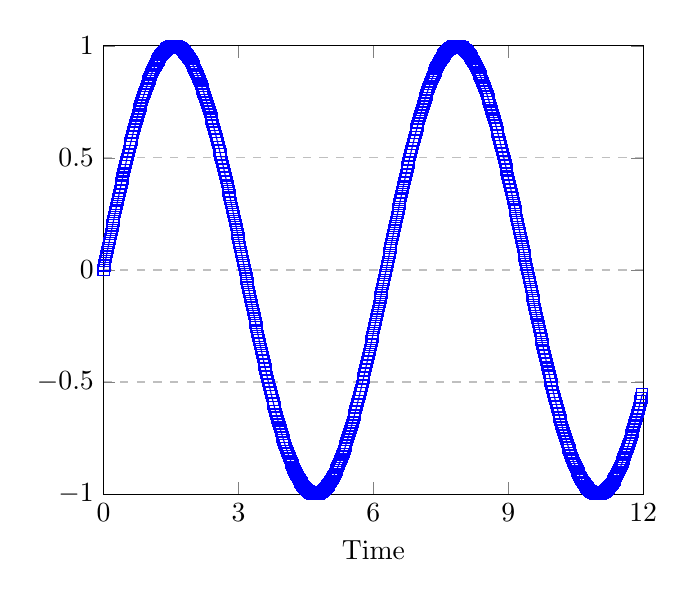
\begin{tikzpicture}
      \begin{axis}[
          xlabel={Time},
          xmin=0, xmax=12,
          ymin=-1, ymax=1,
          xtick={0,3,6,9,12},
          ytick={-1,-0.5,0,0.5,1},
          ymajorgrids=true,
          grid style=dashed,
        ]

        \addplot[
          color=blue,
          mark=square,
        ]
        coordinates {
            (0.000000,0.000000)(0.020000,0.019999)(0.040000,0.039989)(0.060000,0.059964)(0.080000,0.079915)(0.100000,0.099833)(0.120000,0.119712)(0.140000,0.139543)(0.160000,0.159318)(0.180000,0.179030)(0.200000,0.198669)(0.220000,0.218230)(0.240000,0.237703)(0.260000,0.257081)(0.280000,0.276356)(0.300000,0.295520)(0.320000,0.314567)(0.340000,0.333487)(0.360000,0.352274)(0.380000,0.370920)(0.400000,0.389418)(0.420000,0.407760)(0.440000,0.425939)(0.460000,0.443948)(0.480000,0.461779)(0.500000,0.479426)(0.520000,0.496880)(0.540000,0.514136)(0.560000,0.531186)(0.580000,0.548024)(0.600000,0.564642)(0.620000,0.581035)(0.640000,0.597195)(0.660000,0.613117)(0.680000,0.628793)(0.700000,0.644218)(0.720000,0.659385)(0.740000,0.674288)(0.760000,0.688921)(0.780000,0.703279)(0.800000,0.717356)(0.820000,0.731146)(0.840000,0.744643)(0.860000,0.757843)(0.880000,0.770739)(0.900000,0.783327)(0.920000,0.795602)(0.940000,0.807558)(0.960000,0.819192)(0.980000,0.830497)(1.000000,0.841471)(1.020000,0.852108)(1.040000,0.862404)(1.060000,0.872355)(1.080000,0.881958)(1.100000,0.891207)(1.120000,0.900100)(1.140000,0.908633)(1.160000,0.916803)(1.180000,0.924606)(1.200000,0.932039)(1.220000,0.939099)(1.240000,0.945784)(1.260000,0.952090)(1.280000,0.958016)(1.300000,0.963558)(1.320000,0.968715)(1.340000,0.973485)(1.360000,0.977865)(1.380000,0.981854)(1.400000,0.985450)(1.420000,0.988652)(1.440000,0.991458)(1.460000,0.993868)(1.480000,0.995881)(1.500000,0.997495)(1.520000,0.998710)(1.540000,0.999526)(1.560000,0.999942)(1.580000,0.999958)(1.600000,0.999574)(1.620000,0.998790)(1.640000,0.997606)(1.660000,0.996024)(1.680000,0.994043)(1.700000,0.991665)(1.720000,0.988890)(1.740000,0.985719)(1.760000,0.982154)(1.780000,0.978197)(1.800000,0.973848)(1.820000,0.969109)(1.840000,0.963983)(1.860000,0.958471)(1.880000,0.952576)(1.900000,0.946300)(1.920000,0.939645)(1.940000,0.932615)(1.960000,0.925212)(1.980000,0.917438)(2.000000,0.909297)(2.020000,0.900793)(2.040000,0.891929)(2.060000,0.882707)(2.080000,0.873133)(2.100000,0.863209)(2.120000,0.852940)(2.140000,0.842330)(2.160000,0.831383)(2.180000,0.820104)(2.200000,0.808496)(2.220000,0.796565)(2.240000,0.784316)(2.260000,0.771753)(2.280000,0.758881)(2.300000,0.745705)(2.320000,0.732231)(2.340000,0.718465)(2.360000,0.704411)(2.380000,0.690075)(2.400000,0.675463)(2.420000,0.660581)(2.440000,0.645435)(2.460000,0.630031)(2.480000,0.614374)(2.500000,0.598472)(2.520000,0.582331)(2.540000,0.565956)(2.560000,0.549355)(2.580000,0.532535)(2.600000,0.515501)(2.620000,0.498262)(2.640000,0.480823)(2.660000,0.463191)(2.680000,0.445375)(2.700000,0.427380)(2.720000,0.409214)(2.740000,0.390885)(2.760000,0.372399)(2.780000,0.353764)(2.800000,0.334988)(2.820000,0.316078)(2.840000,0.297041)(2.860000,0.277886)(2.880000,0.258619)(2.900000,0.239249)(2.920000,0.219784)(2.940000,0.200230)(2.960000,0.180596)(2.980000,0.160890)(3.000000,0.141120)(3.020000,0.121293)(3.040000,0.101418)(3.060000,0.081502)(3.080000,0.061554)(3.100000,0.041581)(3.120000,0.021591)(3.140000,0.001593)(3.160000,-0.018406)(3.180000,-0.038398)(3.200000,-0.058374)(3.220000,-0.078327)(3.240000,-0.098249)(3.260000,-0.118131)(3.280000,-0.137966)(3.300000,-0.157746)(3.320000,-0.177462)(3.340000,-0.197108)(3.360000,-0.216675)(3.380000,-0.236155)(3.400000,-0.255541)(3.420000,-0.274825)(3.440000,-0.293998)(3.460000,-0.313054)(3.480000,-0.331985)(3.500000,-0.350783)(3.520000,-0.369441)(3.540000,-0.387951)(3.560000,-0.406306)(3.580000,-0.424498)(3.600000,-0.442520)(3.620000,-0.460366)(3.640000,-0.478027)(3.660000,-0.495497)(3.680000,-0.512769)(3.700000,-0.529836)(3.720000,-0.546691)(3.740000,-0.563327)(3.760000,-0.579738)(3.780000,-0.595917)(3.800000,-0.611858)(3.820000,-0.627554)(3.840000,-0.642999)(3.860000,-0.658186)(3.880000,-0.673111)(3.900000,-0.687766)(3.920000,-0.702146)(3.940000,-0.716246)(3.960000,-0.730058)(3.980000,-0.743579)(4.000000,-0.756802)(4.020000,-0.769723)(4.040000,-0.782336)(4.060000,-0.794636)(4.080000,-0.806618)(4.100000,-0.818277)(4.120000,-0.829609)(4.140000,-0.840609)(4.160000,-0.851273)(4.180000,-0.861597)(4.200000,-0.871576)(4.220000,-0.881206)(4.240000,-0.890484)(4.260000,-0.899405)(4.280000,-0.907967)(4.300000,-0.916166)(4.320000,-0.923998)(4.340000,-0.931461)(4.360000,-0.938551)(4.380000,-0.945266)(4.400000,-0.951602)(4.420000,-0.957558)(4.440000,-0.963131)(4.460000,-0.968319)(4.480000,-0.973119)(4.500000,-0.977530)(4.520000,-0.981550)(4.540000,-0.985178)(4.560000,-0.988411)(4.580000,-0.991249)(4.600000,-0.993691)(4.620000,-0.995735)(4.640000,-0.997381)(4.660000,-0.998628)(4.680000,-0.999476)(4.700000,-0.999923)(4.720000,-0.999971)(4.740000,-0.999619)(4.760000,-0.998867)(4.780000,-0.997715)(4.800000,-0.996165)(4.820000,-0.994216)(4.840000,-0.991869)(4.860000,-0.989125)(4.880000,-0.985986)(4.900000,-0.982453)(4.920000,-0.978526)(4.940000,-0.974208)(4.960000,-0.969501)(4.980000,-0.964405)(5.000000,-0.958924)(5.020000,-0.953060)(5.040000,-0.946814)(5.060000,-0.940189)(5.080000,-0.933189)(5.100000,-0.925815)(5.120000,-0.918070)(5.140000,-0.909959)(5.160000,-0.901484)(5.180000,-0.892648)(5.200000,-0.883455)(5.220000,-0.873908)(5.240000,-0.864012)(5.260000,-0.853771)(5.280000,-0.843188)(5.300000,-0.832267)(5.320000,-0.821014)(5.340000,-0.809433)(5.360000,-0.797527)(5.380000,-0.785303)(5.400000,-0.772764)(5.420000,-0.759917)(5.440000,-0.746765)(5.460000,-0.733315)(5.480000,-0.719572)(5.500000,-0.705540)(5.520000,-0.691227)(5.540000,-0.676637)(5.560000,-0.661776)(5.580000,-0.646651)(5.600000,-0.631267)(5.620000,-0.615630)(5.640000,-0.599747)(5.660000,-0.583625)(5.680000,-0.567269)(5.700000,-0.550686)(5.720000,-0.533882)(5.740000,-0.516865)(5.760000,-0.499642)(5.780000,-0.482218)(5.800000,-0.464602)(5.820000,-0.446800)(5.840000,-0.428819)(5.860000,-0.410667)(5.880000,-0.392350)(5.900000,-0.373877)(5.920000,-0.355254)(5.940000,-0.336488)(5.960000,-0.317589)(5.980000,-0.298562)(6.000000,-0.279415)(6.020000,-0.260157)(6.040000,-0.240795)(6.060000,-0.221337)(6.080000,-0.201790)(6.100000,-0.182163)(6.120000,-0.162462)(6.140000,-0.142697)(6.160000,-0.122874)(6.180000,-0.103002)(6.200000,-0.083089)(6.220000,-0.063143)(6.240000,-0.043172)(6.260000,-0.023183)(6.280000,-0.003185)(6.300000,0.016814)(6.320000,0.036806)(6.340000,0.056784)(6.360000,0.076739)(6.380000,0.096664)(6.400000,0.116549)(6.420000,0.136388)(6.440000,0.156173)(6.460000,0.175895)(6.480000,0.195547)(6.500000,0.215120)(6.520000,0.234607)(6.540000,0.254001)(6.560000,0.273293)(6.580000,0.292476)(6.600000,0.311541)(6.620000,0.330482)(6.640000,0.349291)(6.660000,0.367961)(6.680000,0.386483)(6.700000,0.404850)(6.720000,0.423055)(6.740000,0.441092)(6.760000,0.458951)(6.780000,0.476628)(6.800000,0.494113)(6.820000,0.511401)(6.840000,0.528485)(6.860000,0.545357)(6.880000,0.562011)(6.900000,0.578440)(6.920000,0.594637)(6.940000,0.610597)(6.960000,0.626313)(6.980000,0.641778)(7.000000,0.656987)(7.020000,0.671932)(7.040000,0.686609)(7.060000,0.701011)(7.080000,0.715133)(7.100000,0.728969)(7.120000,0.742513)(7.140000,0.755761)(7.160000,0.768705)(7.180000,0.781343)(7.200000,0.793668)(7.220000,0.805675)(7.240000,0.817361)(7.260000,0.828719)(7.280000,0.839746)(7.300000,0.850437)(7.320000,0.860787)(7.340000,0.870794)(7.360000,0.880452)(7.380000,0.889758)(7.400000,0.898708)(7.420000,0.907299)(7.440000,0.915526)(7.460000,0.923388)(7.480000,0.930880)(7.500000,0.938000)(7.520000,0.944745)(7.540000,0.951111)(7.560000,0.957098)(7.580000,0.962701)(7.600000,0.967920)(7.620000,0.972751)(7.640000,0.977193)(7.660000,0.981244)(7.680000,0.984903)(7.700000,0.988168)(7.720000,0.991038)(7.740000,0.993511)(7.760000,0.995587)(7.780000,0.997265)(7.800000,0.998543)(7.820000,0.999423)(7.840000,0.999902)(7.860000,0.999982)(7.880000,0.999662)(7.900000,0.998941)(7.920000,0.997822)(7.940000,0.996303)(7.960000,0.994385)(7.980000,0.992070)(8.000000,0.989358)(8.020000,0.986251)(8.040000,0.982748)(8.060000,0.978853)(8.080000,0.974566)(8.100000,0.969890)(8.120000,0.964825)(8.140000,0.959375)(8.160000,0.953541)(8.180000,0.947325)(8.200000,0.940731)(8.220000,0.933760)(8.240000,0.926415)(8.260000,0.918701)(8.280000,0.910618)(8.300000,0.902172)(8.320000,0.893364)(8.340000,0.884200)(8.360000,0.874681)(8.380000,0.864813)(8.400000,0.854599)(8.420000,0.844043)(8.440000,0.833149)(8.460000,0.821922)(8.480000,0.810367)(8.500000,0.798487)(8.520000,0.786288)(8.540000,0.773774)(8.560000,0.760951)(8.580000,0.747824)(8.600000,0.734397)(8.620000,0.720677)(8.640000,0.706668)(8.660000,0.692377)(8.680000,0.677809)(8.700000,0.662969)(8.720000,0.647865)(8.740000,0.632501)(8.760000,0.616884)(8.780000,0.601021)(8.800000,0.584917)(8.820000,0.568579)(8.840000,0.552014)(8.860000,0.535228)(8.880000,0.518228)(8.900000,0.501021)(8.920000,0.483613)(8.940000,0.466012)(8.960000,0.448224)(8.980000,0.430257)(9.000000,0.412118)(9.020000,0.393815)(9.040000,0.375353)(9.060000,0.356742)(9.080000,0.337988)(9.100000,0.319098)(9.120000,0.300081)(9.140000,0.280944)(9.160000,0.261695)(9.180000,0.242341)(9.200000,0.222890)(9.220000,0.203350)(9.240000,0.183728)(9.260000,0.164033)(9.280000,0.144273)(9.300000,0.124454)(9.320000,0.104586)(9.340000,0.084676)(9.360000,0.064733)(9.380000,0.044763)(9.400000,0.024775)(9.420000,0.004778)(9.440000,-0.015221)(9.460000,-0.035215)(9.480000,-0.055194)(9.500000,-0.075151)(9.520000,-0.095078)(9.540000,-0.114967)(9.560000,-0.134810)(9.580000,-0.154599)(9.600000,-0.174327)(9.620000,-0.193984)(9.640000,-0.213564)(9.660000,-0.233059)(9.680000,-0.252460)(9.700000,-0.271761)(9.720000,-0.290952)(9.740000,-0.310028)(9.760000,-0.328979)(9.780000,-0.347799)(9.800000,-0.366479)(9.820000,-0.385013)(9.840000,-0.403393)(9.860000,-0.421612)(9.880000,-0.439662)(9.900000,-0.457536)(9.920000,-0.475227)(9.940000,-0.492728)(9.960000,-0.510032)(9.980000,-0.527132)(10.000000,-0.544021)(10.020000,-0.560693)(10.040000,-0.577140)(10.060000,-0.593356)(10.080000,-0.609335)(10.100000,-0.625071)(10.120000,-0.640556)(10.140000,-0.655785)(10.160000,-0.670752)(10.180000,-0.685450)(10.200000,-0.699875)(10.220000,-0.714019)(10.240000,-0.727878)(10.260000,-0.741446)(10.280000,-0.754717)(10.300000,-0.767686)(10.320000,-0.780348)(10.340000,-0.792698)(10.360000,-0.804731)(10.380000,-0.816442)(10.400000,-0.827826)(10.420000,-0.838880)(10.440000,-0.849598)(10.460000,-0.859976)(10.480000,-0.870010)(10.500000,-0.879696)(10.520000,-0.889030)(10.540000,-0.898009)(10.560000,-0.906628)(10.580000,-0.914885)(10.600000,-0.922775)(10.620000,-0.930297)(10.640000,-0.937447)(10.660000,-0.944221)(10.680000,-0.950618)(10.700000,-0.956635)(10.720000,-0.962269)(10.740000,-0.967518)(10.760000,-0.972380)(10.780000,-0.976854)(10.800000,-0.980936)(10.820000,-0.984626)(10.840000,-0.987923)(10.860000,-0.990824)(10.880000,-0.993329)(10.900000,-0.995436)(10.920000,-0.997146)(10.940000,-0.998456)(10.960000,-0.999367)(10.980000,-0.999879)(11.000000,-0.999990)(11.020000,-0.999702)(11.040000,-0.999013)(11.060000,-0.997925)(11.080000,-0.996438)(11.100000,-0.994553)(11.120000,-0.992269)(11.140000,-0.989589)(11.160000,-0.986513)(11.180000,-0.983042)(11.200000,-0.979178)(11.220000,-0.974922)(11.240000,-0.970276)(11.260000,-0.965243)(11.280000,-0.959823)(11.300000,-0.954019)(11.320000,-0.947834)(11.340000,-0.941270)(11.360000,-0.934329)(11.380000,-0.927014)(11.400000,-0.919329)(11.420000,-0.911275)(11.440000,-0.902858)(11.460000,-0.894079)(11.480000,-0.884943)(11.500000,-0.875452)(11.520000,-0.865612)(11.540000,-0.855425)(11.560000,-0.844896)(11.580000,-0.834029)(11.600000,-0.822829)(11.620000,-0.811299)(11.640000,-0.799445)(11.660000,-0.787271)(11.680000,-0.774782)(11.700000,-0.761984)(11.720000,-0.748880)(11.740000,-0.735477)(11.760000,-0.721780)(11.780000,-0.707794)(11.800000,-0.693525)(11.820000,-0.678979)(11.840000,-0.664161)(11.860000,-0.649077)(11.880000,-0.633734)(11.900000,-0.618137)(11.920000,-0.602293)(11.940000,-0.586208)(11.960000,-0.569889)(11.980000,-0.553342)
          };

      \end{axis}
    \end{tikzpicture}
  \end{figure}
  For more examples, there is a growing body of documentation that can be found at https://discourse.klank.dev as well as https://github.com/mikesol/purescript-audio-behaviors.

  \subsection{Precise functions of time}

  When using control data to model precise rhythmic events, aliasing will often truncate inflection points, making them arrive to early or too late.  To remedy this, it is possible to specify with sample-rate accuracy (44100 Hz) at what time a value should occur during a control cycle.

  As an example, consider the following audio behavior\footnote{\url{https://klank.dev/?k&url=https://klank-share.s3.eu-west-1.amazonaws.com/K16087041970194799.purs&klank=https://klank-share.s3.eu-west-1.amazonaws.com/klank16087041988326746.js}}:

  \begin{verbatim}
pwf :: Number -> Array (Tuple Number Number)
pwf x =
  join
    $ map
        ( \i ->
            map
              ( \(Tuple f s) ->
                  Tuple (f + x * toNumber i) s
              )
              [ Tuple 0.0 0.0,
              Tuple 0.02 0.7,
              Tuple 0.06 0.2 ]
        )
        (range 0 400)


msBetweenSamples = defaultEngineInfo.msBetweenSamples
kr = (toNumber msBetweenSamples) / 1000.0 :: Number

epwf = evalPiecewise kr

pulse t v p n s =
  gain_' (t <> "go") v
    (gainT_' (t <> "gi")
      (epwf (pwf p) s) $ sinOsc_ (t <> "sw") n)

scene :: Number -> Behavior (AudioUnit D1)
scene s =
  pure
    $ speaker_ "speaker"
        (map (applyFlipped s)
           (pulse "g0" 0.1  0.11 440.0
            :| pulse "g1" 0.1 0.13 660.0 
            : pulse "g2" 0.1 0.15 990.0
            : pulse "g3" 0.1 0.9 220.0
            : pulse "g4" 0.05 0.14 1210.0 
            : pulse "g4" 0.025 0.12 1580.0
            : Nil
        ))
  \end{verbatim}

  The polymetric rhythmic events are placed with audio-rate accuracy using \verb=evalPiecewise=, which is a function that uses \textit{both} time and the control rate to make sure the peaks and troughs of a piecewise function are rendered at the nearest audio-rate sample.

  \begin{figure}[h]
    \caption{Discretized sine wave at a lower control rate causes less-precise extremes and a narrower ambitus, requiring precise event placement between control-rate cycles.}
    \centering
    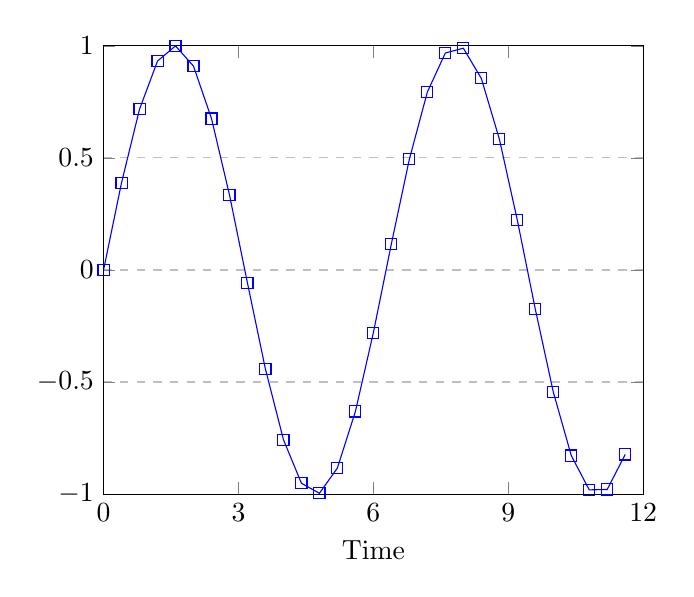
\begin{tikzpicture}
      \begin{axis}[
          xlabel={Time},
          xmin=0, xmax=12,
          ymin=-1, ymax=1,
          xtick={0,3,6,9,12},
          ytick={-1,-0.5,0,0.5,1},
          ymajorgrids=true,
          grid style=dashed,
        ]

        \addplot[
          color=blue,
          mark=square,
        ]
        coordinates {
            (0.000000,0.000000)(0.400000,0.389418)(0.800000,0.717356)(1.200000,0.932039)(1.600000,0.999574)(2.000000,0.909297)(2.400000,0.675463)(2.800000,0.334988)(3.200000,-0.058374)(3.600000,-0.442520)(4.000000,-0.756802)(4.400000,-0.951602)(4.800000,-0.996165)(5.200000,-0.883455)(5.600000,-0.631267)(6.000000,-0.279415)(6.400000,0.116549)(6.800000,0.494113)(7.200000,0.793668)(7.600000,0.967920)(8.000000,0.989358)(8.400000,0.854599)(8.800000,0.584917)(9.200000,0.222890)(9.600000,-0.174327)(10.000000,-0.544021)(10.400000,-0.827826)(10.800000,-0.980936)(11.200000,-0.979178)(11.600000,-0.822829)
          };

      \end{axis}
    \end{tikzpicture}
  \end{figure}

  \subsection{Integration over time}

  The behavior pattern is stateless, which makes it difficult to integrate over time, as an integral (or \verb=fold=) requires remembering an aggregate and modifying it.  As mentioned previously, behaviors are existentially qualified - their signature reads \textit{there exists an \texttt{x} such that, if you give me a function in the form \texttt{(a -> x)}, I'll give you an \texttt{x}}.  The rendering function can parameterize \texttt{x} as a feedback unit that reports previous values (or an initial set of values) and retains new values for a next iteration.

  When working with behaviors, integrals or folds are useful in two contexts:

  \begin{enumerate}
    \item When a function of time is easier to express as a differential equation.  In this case, one can integrate over time to solve the equation.  Phil Freeman's \texttt{purescript-behaviors} library uses this technique for many of the example animations, producing effects like simple harmonic motion.\footnote{https://github.com/paf31/purescript-behaviors}
    \item When a function needs to deal with indeterminacy, ie responding to a user interaction.
  \end{enumerate}

  As an example of the latter, consider the following scene.  When one clicks anywhere with a mouse, the pitch begins to rise linearly. In other words, it integrates over a constant (the slope) with the initial value being the point in time of the click.\footnote{\url{https://klank.dev/?k&ec&url=https://klank-share.s3.amazonaws.com/K1608660252992183.purs&klank=https://klank-share.s3.amazonaws.com/klank16086602569588970.js}}.  To perform the integration, it uses an accumulator of type \verb={ onset :: Maybe Number }=.

  \begin{verbatim}
scene ::
Mouse ->
{ onset :: Maybe Number } ->
CanvasInfo ->
Number ->
Behavior (AV D2 { onset :: Maybe Number })
scene mouse acc@{ onset }
  (CanvasInfo { w, h }) time = f time <$> click
where
f s cl =
  AV
    ( Just
        $ dup1
            ( 
  (gain' 0.1 $ sinOsc 
       (110.0 + (3.0 * sin (0.5 * rad))))
    + ( gain' 0.1
          $ sinOsc
              ( 220.0
                  + ( if cl then (
    50.0
    + maybe 0.0
        (\t -> 30.0 * (s - t))
        stTime
                        )
                      else
                        0.0
                    )
              )
      )
            ) \mono ->
            speaker
              $ ( (panner (-0.5) 
                  (merger
                    (mono +> mono +> empty)))
                    :| Nil
                )
    )
    ( Just
        $ filled
            (fillColor (rgb 0 0 0))
            (circle (w / 2.0)
            (h / 2.0)
            (if cl then 25.0 else 5.0))
    )
    (acc { onset = stTime })
  where
  rad = pi * s

  stTime = case Tuple onset cl of
    (Tuple Nothing true) -> Just s
    (Tuple (Just y) true) -> Just y
    (Tuple _ false) -> Nothing

click :: Behavior Boolean
click = map (not <<< isEmpty) $ buttons mouse
\end{verbatim}

  For a larger example of this integration/accumulator pattern, you can refer to \url{https://bit.ly/silent-night-kdv} (\url{https://bit.ly/silent-night-klank} in developer mode), which uses an accumulator containing information about user interactions to shape the work over time.

  \section{Challenges and initial solutions for FRP web audio}
  Using a stateless functional language like PureScript to model the stateful, imperative WebAudio API presents several challenges.  In this section, I will discuss three difficult aspects of using FRP in web audio along with initial solutions implemented in \texttt{purescript-audio-behaviors}.

  \subsection{Persistent audio units}

  When an audio context is created in JavaScript, it persists until there is no longer a reference to it, at which point the context and all live audio units are destroyed.  The audio context is stateful, meaning that when audio units are connected or disconnected, it retains the state of the audio graph until it is either changed again or destroyed.  In addition to being a useful abstraction for programmers, this also provides the necessary internal memory to nodes like \verb=DelayNode=, \verb=BiquadFilterNode= and \verb=ConvolverNode= that must retain a previous state and/or previous audio.

  The behavior pattern, on the other hand, is stateless: it does not remember what the contents of a prior behavior were.  Even when using an accumulator, there is no way to precisely correlate objects in an audio graph with WebAudio API objects.  For example, consider the following behavior that turns on a second oscillator after 10 seconds.

  \begin{verbatim}
  scene time = pure $
    gain 0.2 (sinOsc 440.0 :|
      (if time > 10.0
        then
        pure (sinOsc 880.0)
        else Nil))
  \end{verbatim}

  There is no information in the graph that would tell the renderer ``do not turn disconnect or reassign the 440Hz oscillator at the ten-second mark.''  The library could choose to assign the previous 440Hz oscillator to the 880Hz oscillator and create a new oscillator at 440Hz.  Or it could choose to destroy the previous oscillator and create two new ones.  All of these scenarios have different sonic properties, but the intent is most likely to persist the 440Hz oscillator to avoid clicks related to change in phase.

  Fortunately, due to the deterministic nature of PureScript's evaluation, it is most often the case that the order of object creation is the same across cycles, leading to a natural persistence of audio units from one cycle to the next.  However, subtle changes can provoke entirely different orders of evaluation, leading to noticeable jank. To mitigate this, one strategy used by many PureScript libraries, including \texttt{purescript-audio-behaviors}, is the \textit{slot} pattern. In the slot pattern, an additional tag of an arbitrary type (often a string) is assigned to each object created.  This tag is then used to group similar objects.  Below, two slots are used to disambiguate the two oscillators:

  \begin{verbatim}
  scene time = pure $
    gain 0.2 (sinOsc_ "osc0" 440.0 :|
      (if time > 10.0
        then pure (sinOsc_ "osc1" 880.0)
        else Nil))
  \end{verbatim}

  \subsection{Front-loaded evaluation}

  The 50Hz control-rate deadline for JavaScript evaluation is more than enough for most simple audio graphs. However, as the graphs get more complicated, 50Hz risks becoming too slow, leading to dropped frames.

  One way to solve this issue is to pre-compile as much of the graph as possible as an array that can be indexed by time, very much like a lookup table for sine waves, but at the audio-graph scale. For instance, the previous pulse example can be almost entirely pre-compiled, as it stops computation after 400 iterations.  That leads to a 97\% reduction in evaluation time of the graph at the expense of upfront compilation time.  The reduction becomes more substantial as the graph becomes larger \footnote{\url{https://klank.dev/?k&url=https://klank-share.s3.amazonaws.com/K16087046614232954.purs&klank=https://klank-share.s3.amazonaws.com/klank16087046653836736.js}}.

  \begin{verbatim}
maxPulse = 18000 :: Int

pwf :: Number -> Array (Tuple Number Number)
pwf x =
  join
    $ map
        ( \i ->
            map
              ( \(Tuple f s) ->
                  Tuple (f + x * toNumber i) s
              )
              [ Tuple 0.0 0.0
              , Tuple 0.02 0.7
              , Tuple 0.06 0.2
              ]
        )
        (range 0 400)

kr =
  (toNumber defaultEngineInfo.msBetweenSamples)
    / 1000.0 ::
    Number

epwf ::
  Array (Tuple Number Number) ->
  Number ->
  AudioParameter
epwf = evalPiecewise kr

pulse t v p n s =
  gain_' (t <> "go") v
    ( gainT_' (t <> "gi")
        (epwf (pwf p) s)
        $ sinOsc_ (t <> "sw") n
    )

makeGraph :: Number -> AudioUnit D1
makeGraph s =
  speaker_ "speaker"
    ( map (applyFlipped s)
        ( pulse "g0" 0.1 0.11 440.0
            :| pulse "g1" 0.1 0.13 660.0
            : pulse "g2" 0.1 0.15 990.0
            : pulse "g3" 0.1 0.9 220.0
            : pulse "g4" 0.05 0.14 1210.0
            : pulse "g4" 0.025 0.12 1580.0
            : Nil
        )
    )

pulses :: Array (AudioUnit D1)
pulses =
  map
    (makeGraph <<< (_ * kr) <<< toNumber)
    (range 0 maxPulse)

defaultGraph :: AudioUnit D1
defaultGraph = makeGraph (toNumber maxPulse * kr)

getPulse :: Number -> AudioUnit D1
getPulse time =
  fromMaybe defaultGraph
    $ index pulses (floor $ time / kr)

scene :: Number -> Behavior (AudioUnit D1)
scene = pure <<< getPulse
  \end{verbatim}

  \subsection{Scheduling}

  As is the case with all realtime audio processing, Web Audio scheduling must achieve a balance between look-ahead, which safeguards against dropped frames, and JIT evaluation, which allows for reactive responses to user input.\cite{schnell2015time}\cite{pendharkar2015adventures} There is no silver-bullet to achieve low-millisecond responsiveness without dropped frames, and the audio graph will only be as responsive as:

  \begin{itemize}
    \item The periodicity of the polling function discussed in Section 1. In most real-world applications, 20 milliseconds is an achievable gap between polls.
    \item The amount of time it takes to build the graph and report it to the web-audio API.  By definition, this should not exceed the amount of time between polls, and ideally should be less (ie 15 milliseconds).
    \item The amount of look-ahead time, which is often 20-40 milliseconds.
  \end{itemize}

  This leads to a delay of ~60-80 milliseconds for responsive input, which is almost always perceptible.\footnote{See \url{https://twitter.com/stronglynormal/status/1326136187116023812} and \url{https://twitter.com/stronglynormal/status/1316756584786276352} for examples of this latency} For mouse clicks, this tends to be less obvious, as psychologically we expect to see the results of a click only after lifting the mouse, whereas processing can start on a \texttt{mousedown} event. However, for MIDI events, this is longer than the minimum latency needed for musicians to feel comfortable playing a digital instrument (roughly 15ms).\cite{jack2018action}

  In \texttt{purescript-audio-behaviors}, there is ongoing work to improve audio scheduling so that it achieves the 15 millisecond deadline needed for real world musical instruments.  This includes:

  \begin{itemize}
    \item Using event listeners to trigger the construction of the audio graph in addition to a pure polling solution. This eliminates the 20ms of between-poll latency, achieving sub-millisecond triggering of the graph construction.
    \item By pre-rendering substantial chunks of the graph, the building of the audio graph can take less than 10ms.  It is possible to shrink this time even further by pushing the pre-rendering to include the list of imperative, assembly-like instructions given directly to the WebAudio API.
    \item Including instructions to ignore look-ahead rendering for certain events, scheduling them for immediate execution.
  \end{itemize}

  These changes are intended to be part of the \texttt{0.0.0} release of \texttt{purescript-audio-behaviors} that will hopefully arrive in mid-2021.

  \section{Conclusions}
  FRP and the \textit{behavior pattern} is an attractive way to turn the imperative WebAudio API into a declarative data structure that is calculated as a function of several input streams such as the \verb=currentTime= of the audio context, mouse events and MIDI-events.  Because the behavior pattern requires the construction of an entire audio graph based on polling, it tends to be ill-suited to reactive, realtime audio applications.  This can be mitigated by several strategies, including using the DOM's native event listeners, pre-compiling substantial parts of the graph and mixing look-ahead with immediate execution.
  %\end{document}  % This is where a 'short' article might terminate

  %ACKNOWLEDGMENTS are optional
  \section{Acknowledgments}
  I'd like to thank Phil Freeman for creating both PureScript and \texttt{purescript-behaviors}, without which this paper would not have been possible.  I'd also like to thank the PureScript community for their helpful answers to my questions as I learned the language and built \texttt{purescript-audio-behaviors}.

  %
  % The following two commands are all you need in the
  % initial runs of your .tex file to
  % produce the bibliography for the citations in your paper.
  \bibliographystyle{abbrv}
  \bibliography{sigproc}  % sigproc.bib is the name of the Bibliography in this case

\end{sloppypar}
\end{document}
